% SPDX-FileCopyrightText: 2026 Bart van de Lint
% SPDX-License-Identifier: AGPL-3.0-or-later
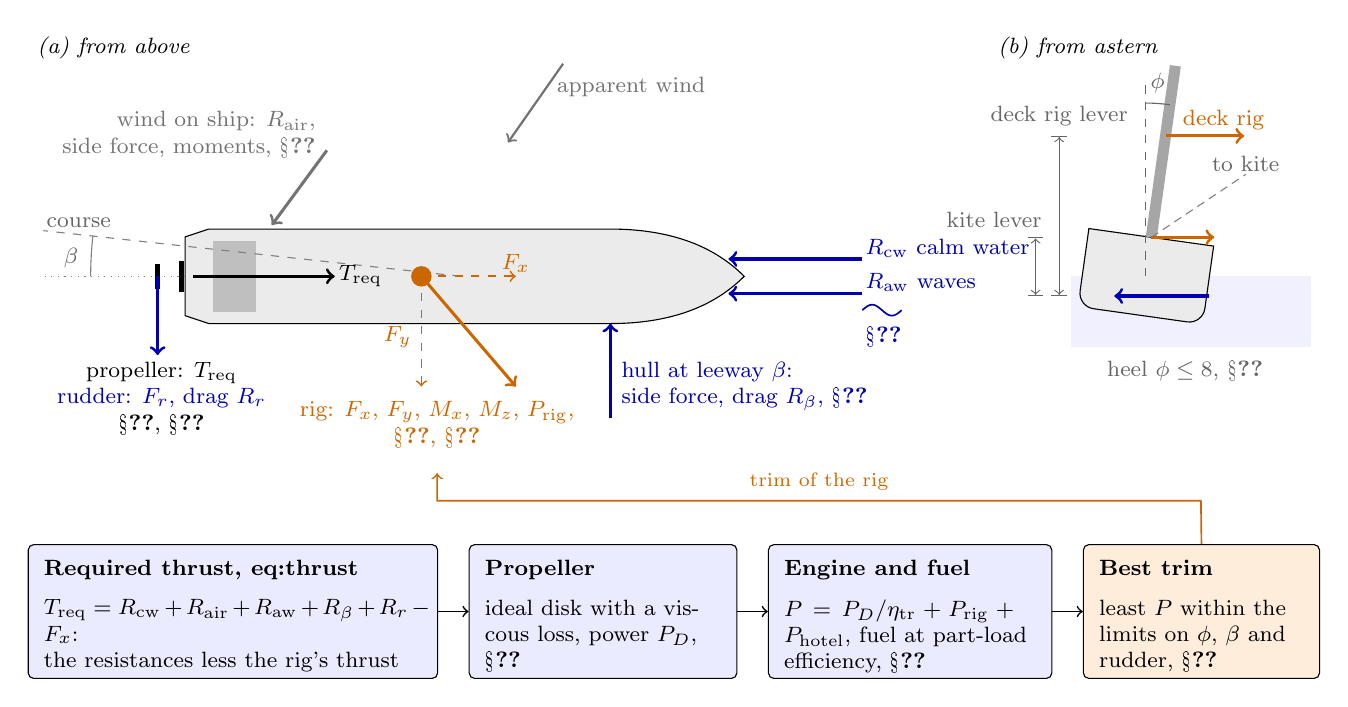
\begin{tikzpicture}[x=1mm, y=1mm, font=\footnotesize,
  water/.style={blue!70!black}, air/.style={black!55}, rig/.style={orange!80!black},
  force/.style={->, line width=1.1pt},
  part/.style={align=left, inner sep=1pt},
  box/.style={draw, rounded corners=2pt, minimum height=17mm, inner sep=0pt},
  boxtitle/.style={font=\footnotesize\bfseries, anchor=north west, inner sep=0pt},
  boxtext/.style={align=left, anchor=north west, inner sep=0pt},
  shipc/.style={fill=blue!8}, rigc/.style={fill=orange!14},
  arrow/.style={->, semithick},
]
% ---- from above, bow to the right; the wind comes from the top
\node[font=\footnotesize\itshape, anchor=west] at (0,29) {(a) from above};
\draw[fill=black!8] (20,-5) -- (23,-6) -- (74,-6) .. controls (83,-6) and (88,-3) .. (91,0)
  .. controls (88,3) and (83,6) .. (74,6) -- (23,6) -- (20,5) -- cycle;
\fill[black!25] (23.5,-4.5) rectangle (29,4.5);
\draw[air, ->, thick] (68,27) -- (61,17) node[pos=0.3, right] {apparent wind};
% leeway: the heading against the course through the water
\draw[black!50, dotted] (20,0) -- (2,0);
\draw[black!50, dashed] (55,0) -- (2,5.8);
\draw[black!50] (8,0) arc[start angle=180, end angle=173.7, radius=47];
\node[black!60] at (5.5,2.3) {$\beta$};
\node[black!60, anchor=south west, inner sep=1pt] at (2,5.8) {course};
% propeller and rudder
\fill[black] (19.2,-2) rectangle (19.8,2);
\draw[line width=1.6pt] (16.5,-1.6) -- (16.5,1.6);
\draw[force] (21,0) -- (39,0) node[right, inner sep=1pt] {$T_\mathrm{req}$};
\draw[force, water] (16.5,0) -- (16.5,-10);
\node[part, anchor=north, align=center] at (17,-10.5) {propeller: $T_\mathrm{req}$\\ \textcolor{blue!70!black}{rudder: $F_r$, drag $R_r$}\\ \S\ref{sec:ships}, \S\ref{sec:balance}};
% wind on the ship
\draw[force, air] (38,16) -- (31,6.5);
\node[part, air, anchor=east, align=right] at (37,18) {wind on ship: $R_\mathrm{air}$,\\ side force, moments, \S\ref{sec:ships}};
% rig
\fill[rig] (50,0) circle (1.3);
\draw[rig, dashed, ->, semithick] (50,0) -- (62,0) node[above, rig, inner sep=1pt] {$F_x$};
\draw[rig, dashed, ->, semithick] (50,0) -- (50,-14) node[pos=0.55, left, rig] {$F_y$};
\draw[force, rig] (50,0) -- (62,-14);
\node[part, rig, anchor=north, align=center] at (52,-15.5) {rig: $F_x$, $F_y$, $M_x$, $M_z$, $P_\mathrm{rig}$,\\ \S\ref{sec:deck_rigs}, \S\ref{sec:kite}};
% hull at leeway
\draw[force, water] (74,-18) -- (74,-6);
\node[part, water, anchor=west] at (75,-14) {hull at leeway $\beta$:\\ side force, drag $R_\beta$, \S\ref{sec:balance}};
% resistances on the bow
\draw[force, water] (106,2.2) -- (89,2.2);
\draw[force, water] (106,-2.2) -- (89,-2.2);
\draw[water, semithick] (106,-4.3) sin (107.25,-3.6) cos (108.5,-4.3) sin (109.75,-5) cos (111,-4.3);
\node[part, water, anchor=west] at (106,3.6) {$R_\mathrm{cw}$ calm water};
\node[part, water, anchor=west] at (106,-0.8) {$R_\mathrm{aw}$ waves};
\node[part, water, anchor=north west] at (106,-6) {\S\ref{sec:ships}};
% ---- from astern, heeled to leeward: wing sail or rotor against kite
\node[font=\footnotesize\itshape, anchor=west] at (122,29) {(b) from astern};
\begin{scope}[shift={(142,0)}]
  \fill[blue!6] (-9.5,-9) rectangle (21,0);
  \begin{scope}[rotate=-8]
    \draw[fill=black!8] (-8,5) -- (-8,-3) arc[start angle=180, end angle=270, radius=2]
      -- (6,-5) arc[start angle=270, end angle=360, radius=2] -- (8,5) -- cycle;
    \fill[black!35] (-0.7,5) rectangle (0.7,27);
    \coordinate (wing) at (0,18);
    \coordinate (tow) at (0,5);
  \end{scope}
  \draw[black!60, dashed] (0,0) -- (0,25);
  \draw[black!60] (0,22) arc[start angle=90, end angle=82, radius=22];
  \node[black!60] at (1.5,24.5) {$\phi$};
  \draw[black!50, densely dashed] (tow) -- ++(12,8) node[above, black!60, inner sep=1pt] {to kite};
  \draw[force, rig] (wing) -- ++(10,0);
  \node[part, rig, anchor=south west] at ([shift={(1.8,0.3)}]wing) {deck rig};
  \draw[force, rig] (tow) -- ++(8,0);
  \draw[force, water] (8,-2.5) -- (-4,-2.5);
  \draw[black!60, |<->|] (-11,-2.5) -- (-11,0 |- wing) node[above] {deck rig lever};
  \draw[black!60, |<->|] (-14,-2.5) -- (-14,0 |- tow) node[above left, xshift=2mm] {kite lever};
  \node[black!60, anchor=north] at (5,-9.5) {heel $\phi\le\SI{8}{\degree}$, \S\ref{sec:balance}};
\end{scope}
% ---- how the parts combine
\pgfmathsetmacro{\rowy}{-34}
\node[box, shipc, minimum width=52mm, anchor=north west] (thrust) at (0,\rowy) {};
\node[boxtitle] at ([shift={(2,-2)}]thrust.north west) {Required thrust, \cref{eq:thrust}};
\node[boxtext, text width=49mm] at ([shift={(2,-7)}]thrust.north west) {$T_\mathrm{req} = R_\mathrm{cw} + R_\mathrm{air} + R_\mathrm{aw} + R_\beta + R_r - F_x$:\\ the resistances less the rig's thrust};
\node[box, shipc, minimum width=34mm, anchor=north west] (prop) at (56,\rowy) {};
\node[boxtitle] at ([shift={(2,-2)}]prop.north west) {Propeller};
\node[boxtext, text width=31mm] at ([shift={(2,-7)}]prop.north west) {ideal disk with a viscous loss, power $P_D$, \S\ref{sec:ships}};
\node[box, shipc, minimum width=36mm, anchor=north west] (engine) at (94,\rowy) {};
\node[boxtitle] at ([shift={(2,-2)}]engine.north west) {Engine and fuel};
\node[boxtext, text width=33mm] at ([shift={(2,-7)}]engine.north west) {$P = P_D/\eta_\mathrm{tr} + P_\mathrm{rig} + P_\mathrm{hotel}$, fuel at part-load efficiency, \S\ref{sec:ships}};
\node[box, rigc, minimum width=30mm, anchor=north west] (trim) at (134,\rowy) {};
\node[boxtitle] at ([shift={(2,-2)}]trim.north west) {Best trim};
\node[boxtext, text width=27mm] at ([shift={(2,-7)}]trim.north west) {least $P$ within the limits on $\phi$, $\beta$ and rudder, \S\ref{sec:balance}};
\draw[arrow] (thrust) -- (prop);
\draw[arrow] (prop) -- (engine);
\draw[arrow] (engine) -- (trim);
\draw[arrow, rig] (trim.north) -- (149,-28.5) -| node[pos=0.25, above, font=\scriptsize] {trim of the rig} (52,-25);
\end{tikzpicture}
